% ============================================================
% LaTeX figure/table includes — auto-generated by paper-figure
% Paper: Interpretable Geometric Features Reveal the
%        Information Bottleneck in RNA Inverse Folding
% Date: 2026-05-18
% ============================================================

% === Fig 1: Hero Figure (Phase 2b — figure-spec) ===
\begin{figure}[t]
    \centering
    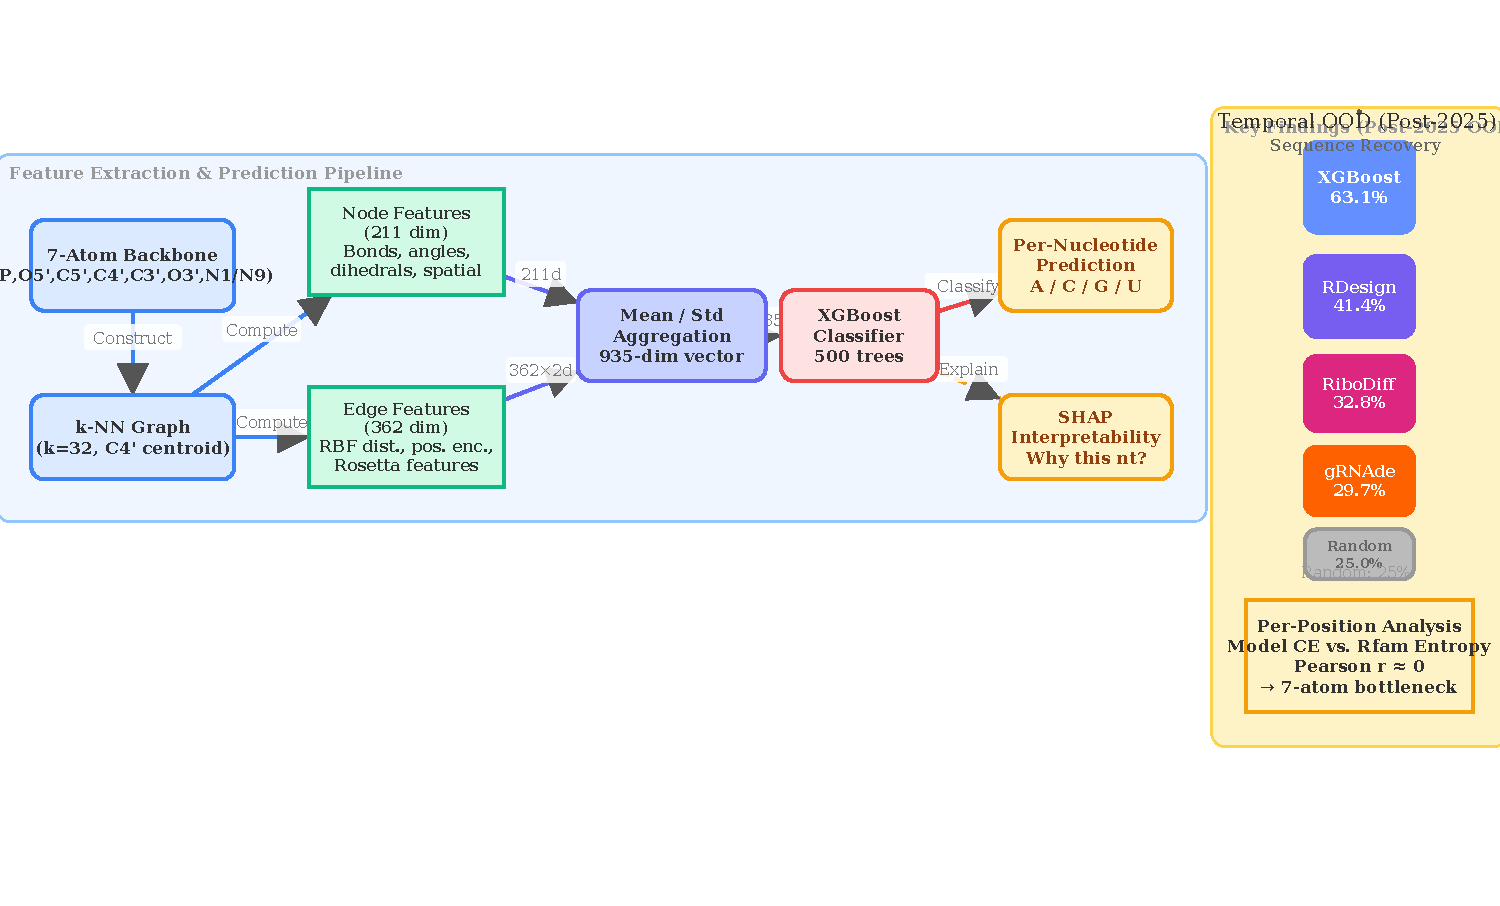
\includegraphics[width=0.78\textwidth]{figures/fig1_hero_architecture.pdf}
    \caption{Overview of the interpretable geometric feature framework
    for RNA inverse folding. \textbf{(Left)} From 7-atom coarse-grained
    backbone coordinates, we compute 935 explicit geometric features
    (211 node + 724 edge-derived) per nucleotide and train an XGBoost
    classifier with per-prediction SHAP interpretability.
    \textbf{(Right)} Key findings: physics-anchored features remain
    stable on post-2025 structures while learned representations
    collapse (top); model errors are uncorrelated with evolutionary
    conservation, proving the 7-atom representation is the information
    bottleneck (bottom).}
    \label{fig:hero}
\end{figure}


% === Fig 3: Temporal OOD Comparison ===
\begin{figure}[t]
    \centering
    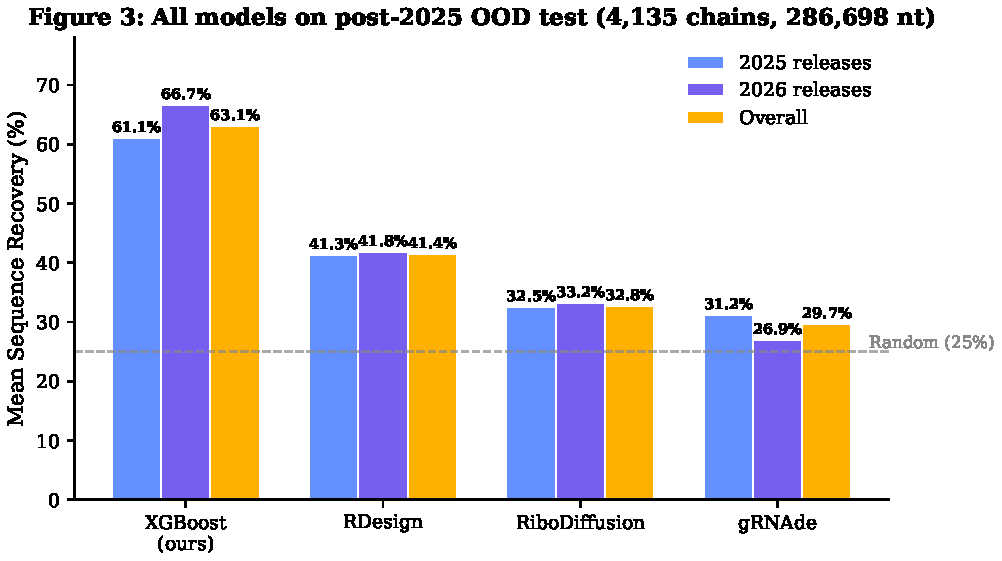
\includegraphics[width=0.75\textwidth]{figures/fig3_temporal_ood.pdf}
    \caption{All models evaluated on the identical post-2025 OOD test
    set (4,135 chains, 286,698 nt). Results split by release year
    (2025, 2026) and overall. XGBoost maintains 63.1\% mean recovery
    while learned representations collapse: gRNAde drops 26 pp from
    its published 56\% to 29.7\%. The dashed line marks random
    baseline (25\%).}
    \label{fig:temporal_ood}
\end{figure}


% === Fig 5: Per-Family Heatmap ===
\begin{figure}[t]
    \centering
    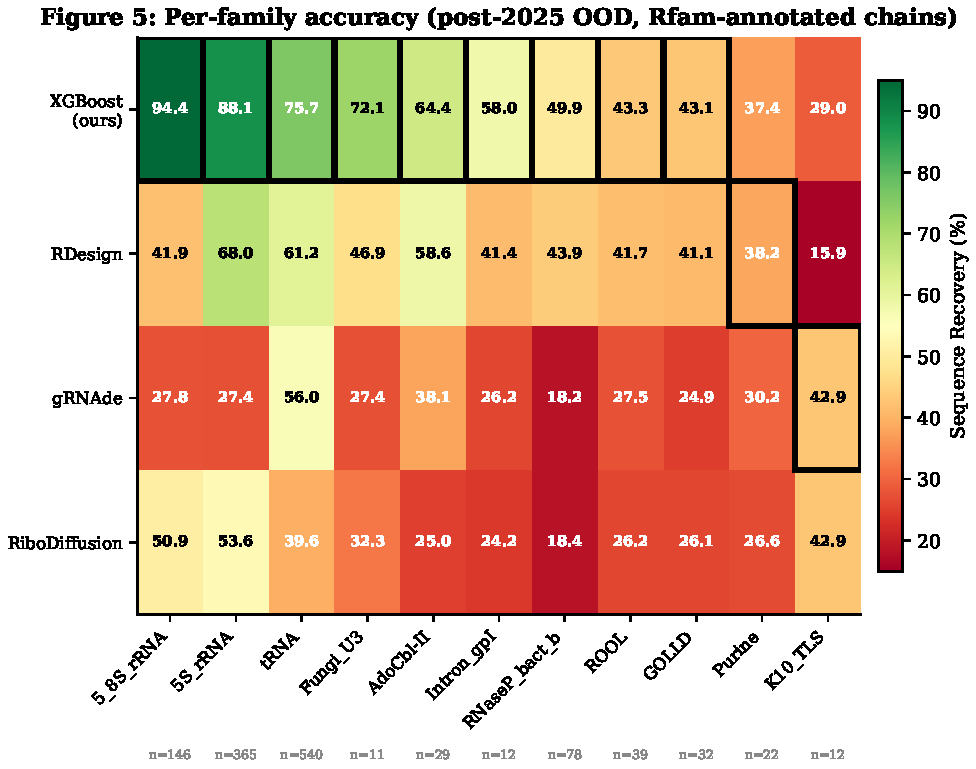
\includegraphics[width=0.75\textwidth]{figures/fig5_per_family_heatmap.pdf}
    \caption{Per-family sequence recovery on post-2025 OOD
    Rfam-annotated chains (11 families with $\geq$10 chains).
    Color intensity indicates accuracy; black borders mark the
    best model per family. XGBoost leads on 9 of 11 families.
    Ribosomal RNAs (5\_8S\_rRNA, 5S\_rRNA) are highly predictable
    ($>$88\%); small riboswitches (Purine, K10\_TLS) remain
    challenging ($<$43\%). Chain counts shown above each family.}
    \label{fig:per_family}
\end{figure}


% === Fig 6: Entropy Scatter ===
\begin{figure}[t]
    \centering
    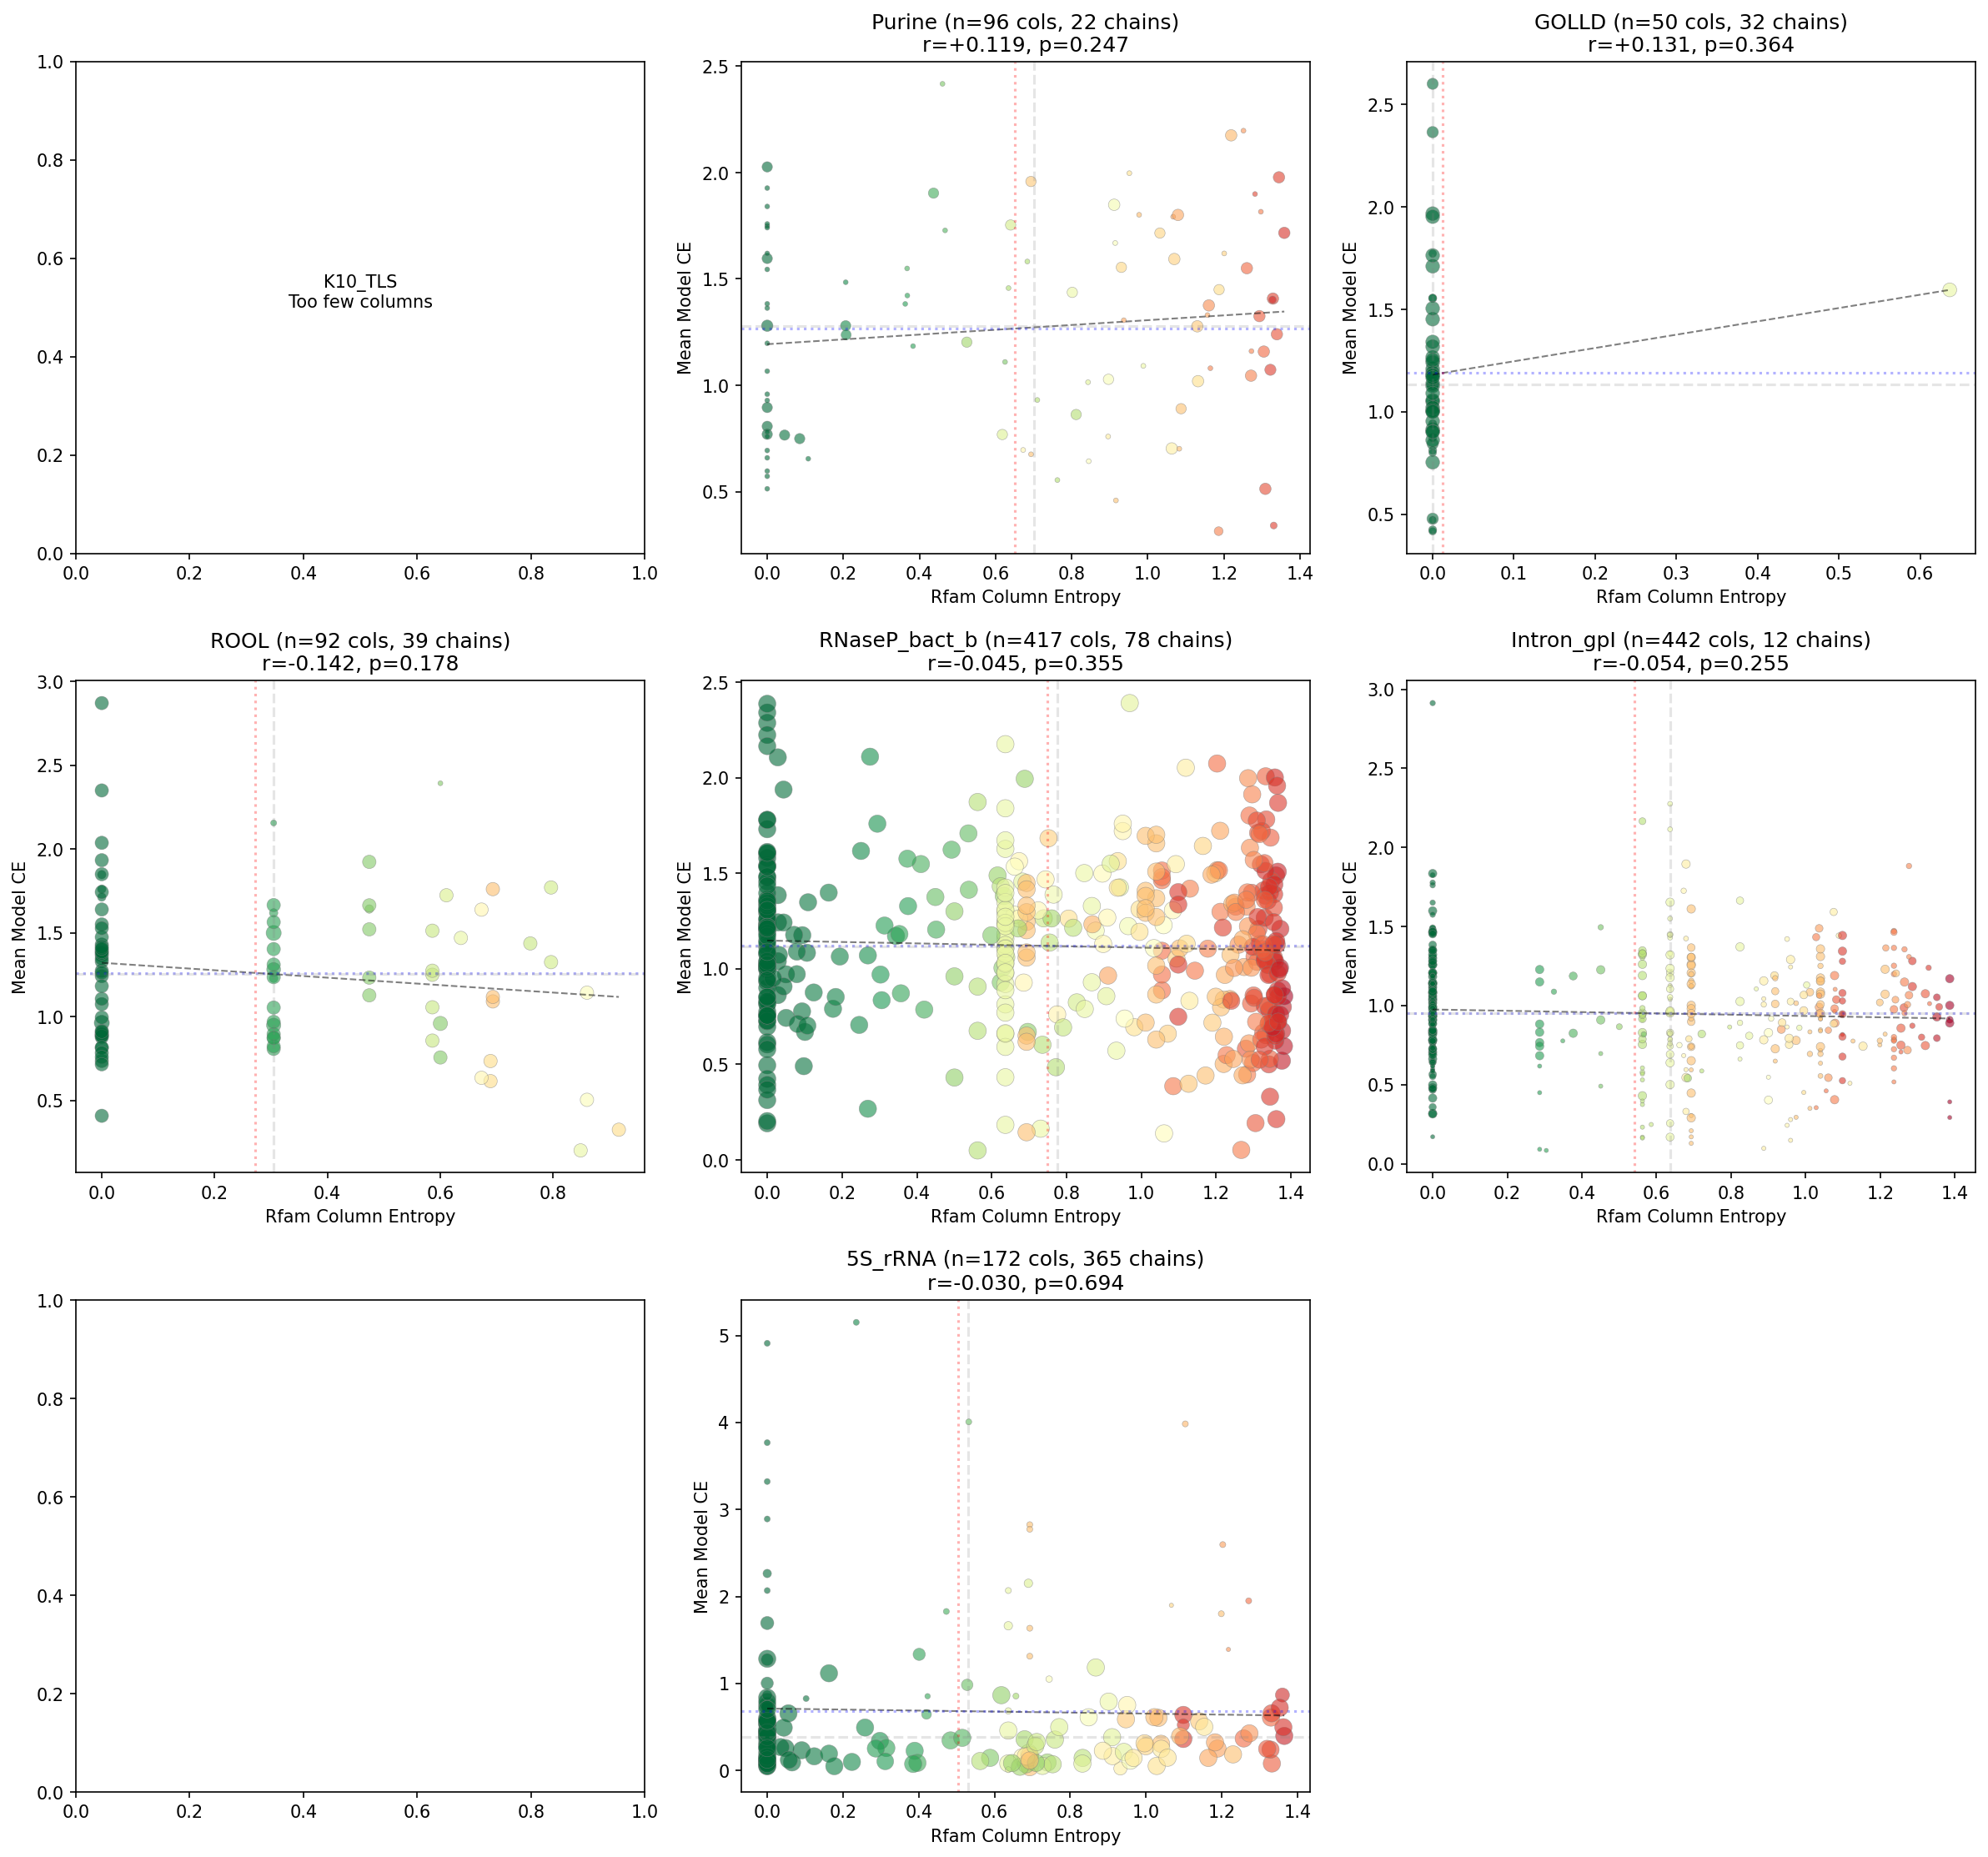
\includegraphics[width=0.75\textwidth]{figures/fig6_entropy_scatter.png}
    \caption{Per-position model cross-entropy vs.\ Rfam evolutionary
    column entropy for 9 Rfam families with sufficient seed alignment
    data. Each point represents one aligned column. Pearson $r$ values
    (annotated per panel) range from $-$0.14 to $+$0.25, confirming
    that model errors are uncorrelated with evolutionary variability.
    High-CE errors at perfectly conserved positions (Rfam entropy = 0)
    indicate that the 7-atom backbone lacks the chemical information
    needed for discrimination --- a representation bottleneck, not a
    model capacity limitation.}
    \label{fig:entropy}
\end{figure}


% === Fig 7: SHAP Importance ===
\begin{figure}[t]
    \centering
    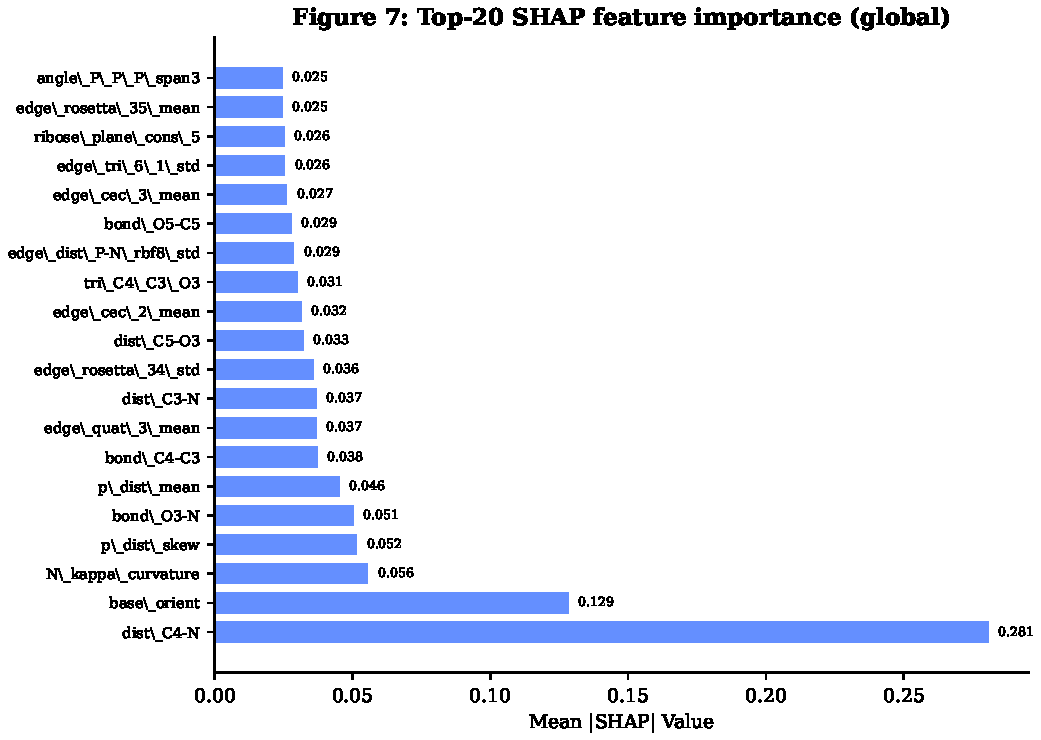
\includegraphics[width=0.72\textwidth]{figures/fig7_shap_importance.pdf}
    \caption{Top-20 global SHAP feature importance scores. The
    glycosidic nitrogen distance (\texttt{dist\_C4-N}) dominates,
    followed by base orientation and curvature features. Bond
    lengths and edge-derived spatial statistics provide complementary
    signals. Per-class analysis reveals chemically meaningful
    differences (see \S\ref{sec:discussion}).}
    \label{fig:shap}
\end{figure}
